\documentclass[12pt,a4paper]{article}

\usepackage[utf8]{inputenc}
\usepackage[T1]{fontenc}
\usepackage{lmodern}
\usepackage[brazilian]{babel}
\usepackage[margin=2.5cm]{geometry}
\usepackage{graphicx}
\usepackage{booktabs}
\usepackage{array}
\newcolumntype{L}[1]{>{\raggedright\arraybackslash}p{#1}}
\usepackage{float}
\usepackage[section]{placeins}
\usepackage{url}
\usepackage{indentfirst}
\usepackage{xcolor}
\usepackage{caption}
\usepackage{listings}
\usepackage[hidelinks]{hyperref}

\graphicspath{{diagramas/}}

\renewcommand{\topfraction}{0.85}
\renewcommand{\textfraction}{0.1}
\renewcommand{\floatpagefraction}{0.75}

\renewcommand{\lstlistingname}{Código}
\renewcommand{\lstlistlistingname}{Lista de códigos}

\lstset{
  language=Java,
  basicstyle=\ttfamily\footnotesize,
  keywordstyle=\color{blue!60!black}\bfseries,
  stringstyle=\color{green!40!black},
  commentstyle=\color{gray},
  frame=single,
  rulecolor=\color{gray!50},
  breaklines=true,
  showstringspaces=false,
  columns=fullflexible,
  keepspaces=true,
  captionpos=b,
  literate=
    {á}{{\'a}}1 {à}{{\`a}}1 {â}{{\^a}}1 {ã}{{\~a}}1
    {é}{{\'e}}1 {ê}{{\^e}}1 {í}{{\'i}}1
    {ó}{{\'o}}1 {ô}{{\^o}}1 {õ}{{\~o}}1 {ú}{{\'u}}1
    {ç}{{\c{c}}}1 {Á}{{\'A}}1 {É}{{\'E}}1 {Ç}{{\c{C}}}1
}


\title{\textbf{Sistema de Vagas do Shopping}\\[4pt]
\large Descrição Arquitetural --- Parte 2: o problema, o sistema e as suas preocupações}
\author{Grupo 4: [PREENCHER: integrantes]}
\date{Arquitetura e Padrões de Software --- 2026.2 --- [PREENCHER: turma]\\
Professor(a): [PREENCHER]\\[4pt]
Novembro de 2026}

\begin{document}
\maketitle

\begin{abstract}
Este documento apresenta o problema que motivou o sistema de gerenciamento das vagas de estacionamento de um shopping e descreve o sistema construído como solução, na arquitetura de memória compartilhada \emph{Blackboard}. Seguindo a norma ISO/IEC/IEEE 42010 e o catálogo de Rozanski e Woods, o texto identifica as partes interessadas e as suas preocupações, descreve o sistema por sete pontos de vista (contexto, funcional, informação, concorrência, desenvolvimento, implantação e operacional) e o examina por seis perspectivas de qualidade (evolução, desempenho, disponibilidade, segurança e privacidade, usabilidade e regulação). No fim, registra as principais decisões arquiteturais, a rastreabilidade até o enunciado do trabalho e as limitações do protótipo. Os padrões de software usados são tratados num documento à parte (Parte 1).
\end{abstract}

\section{Introdução}

Uma \textbf{descrição arquitetural} explica como um sistema está organizado e por quê, para as pessoas que precisam entendê-lo, construí-lo, operá-lo ou avaliá-lo. A norma ISO/IEC/IEEE 42010~\cite{iso42010} organiza essa descrição em quatro ideias:

\begin{itemize}
  \item \textbf{partes interessadas} (\emph{stakeholders}): as pessoas, grupos ou organizações que têm interesse no sistema, como o operador da cancela ou a gerência do shopping;
  \item \textbf{preocupações} (\emph{concerns}): o que importa para cada parte interessada, por exemplo ``saber, a qualquer momento, quantas vagas estão livres'';
  \item \textbf{pontos de vista} (\emph{viewpoints}): as convenções para olhar o sistema de um certo ângulo, com os modelos e diagramas adequados a esse ângulo;
  \item \textbf{visões} (\emph{views}): o sistema descrito segundo um ponto de vista; cada visão trata de algumas preocupações.
\end{itemize}

Rozanski e Woods~\cite{rozanski2011} propõem um catálogo de sete pontos de vista e acrescentam as \textbf{perspectivas}: qualidades que atravessam várias visões ao mesmo tempo, como a segurança ou o desempenho. Uma perspectiva não gera um diagrama novo; ela é uma pergunta aplicada a todas as visões (``o que, nesta visão, afeta a privacidade?'').

Este documento usa essa estrutura. A Seção~\ref{sec:problema} cria o problema, e a Seção~\ref{sec:solucao} apresenta o sistema como solução. A Seção~\ref{sec:preocupacoes} lista as partes interessadas e as preocupações. As Seções~\ref{sec:pontos} e~\ref{sec:perspectivas} descrevem os pontos de vista e as perspectivas que tratam essas preocupações. As Seções~\ref{sec:decisoes} a~\ref{sec:limitacoes} registram as decisões, a rastreabilidade e as limitações. Os diagramas completos (implantação, casos de uso, atividades, estados e classes) acompanham este documento na pasta \texttt{diagramas}, e os padrões de software estão descritos na Parte~1.

\section{O problema}
\label{sec:problema}

O cenário é fictício. Um shopping center tem um estacionamento com dois setores:

\begin{itemize}
  \item o \textbf{Externo}, ao ar livre, com 15 vagas comuns (fileiras A a C, posições 1 a 5);
  \item o \textbf{Subsolo}, coberto, com 10 vagas (fileiras A e B, posições 1 a 5). O teto baixo limita a altura dos veículos a 2,10~m, e as vagas A1 e A2 são preferenciais, reservadas a quem tem um motivo de uso (por exemplo, pessoa idosa, pessoa com deficiência ou gestante).
\end{itemize}

Hoje, o controle é feito de forma manual, e isso causa cinco problemas:

\begin{enumerate}
  \item \textbf{Ninguém sabe quantas vagas estão livres.} O motorista entra e circula pelo setor procurando vaga, e o operador da cancela não sabe se deve orientá-lo para o outro setor.
  \item \textbf{Veículos altos entram no Subsolo.} Sem conferir a altura na cancela, uma caminhonete ou uma van com bagageiro pode bater no teto ou ficar presa na rampa.
  \item \textbf{As vagas preferenciais são usadas sem motivo.} Não há registro de quem ocupou a vaga, nem do motivo declarado, o que impede a fiscalização.
  \item \textbf{A gerência não tem dados.} Não se sabe em que horários o estacionamento lota, quanto tempo os clientes ficam, quais vagas giram mais nem quais clientes voltam com frequência. Decisões como ampliar um setor ou mudar o horário das equipes são tomadas sem informação.
  \item \textbf{O pouco que se registra se perde.} Anotações em papel ou em planilhas soltas não sobrevivem à troca de turno nem permitem consultas por placa ou por período.
\end{enumerate}

\section{O sistema como solução}
\label{sec:solucao}

\subsection{Visão geral}

O sistema registra a passagem de cada veículo por quatro eventos: a \textbf{entrada} na cancela do setor, a \textbf{ocupação} de uma vaga, a \textbf{desocupação} da vaga e a \textbf{saída} pela cancela. Entre a entrada e a ocupação, e entre a desocupação e a saída, o veículo está \emph{circulando} no setor; entre a ocupação e a desocupação, está \emph{estacionado}.

A organização segue o padrão Blackboard, pedido pelo enunciado. Um quadro central (o \emph{Blackboard}) guarda as vagas, o histórico de cada passagem e as requisições em andamento. Três especialistas independentes trabalham sobre esse quadro:

\begin{itemize}
  \item o especialista do \textbf{Externo} e o do \textbf{Subsolo} validam e registram os quatro eventos de cada setor, com as regras próprias de cada um (no Subsolo, a altura máxima e o motivo nas vagas preferenciais);
  \item o especialista de \textbf{relatórios} analisa o histórico e produz onze relatórios para a gerência, como a ocupação por setor, os horários de pico, os clientes frequentes e o giro por vaga.
\end{itemize}

Os especialistas não se comunicam entre si: cada um lê e escreve apenas no quadro. Um componente de controle recebe cada requisição e escolhe o especialista que deve tratá-la.

O operador usa uma janela com o mapa das vagas de cada setor (verde para livre, azul para preferencial livre, vermelho para ocupada), a lista dos veículos circulando e um painel que mostra, a cada requisição, qual especialista respondeu e o resultado. Há também uma interface de texto, para terminais sem tela gráfica. Cada evento aceito é gravado num arquivo CSV, relido quando o programa abre, e um cenário pronto com uma semana de uso fictício permite demonstrar os relatórios.

\subsection{Escopo}

O sistema faz:
\begin{itemize}
  \item o registro dos quatro eventos, com as recusas explicadas (por exemplo, ``o veículo ainda ocupa a vaga A3; registre a desocupação antes da saída'');
  \item a conferência da altura na entrada do Subsolo e do motivo nas vagas preferenciais;
  \item o mapa das vagas em tempo real e a lista dos veículos que procuram vaga;
  \item onze relatórios gerenciais, inclusive por placa e por período;
  \item a gravação do uso num arquivo e a sua releitura ao abrir o programa;
  \item o carregamento de um cenário de demonstração e a opção de zerar os dados.
\end{itemize}

Ficam fora do escopo do protótipo:
\begin{itemize}
  \item a cobrança e o cálculo de tarifas;
  \item a integração com cancelas, sensores de vaga e leitura automática de placas: no protótipo, o operador faz o papel desses equipamentos;
  \item o uso por vários computadores ao mesmo tempo, em rede;
  \item o controle de acesso por usuário e a política de retenção dos dados (tratados como limitações na Seção~\ref{sec:limitacoes}).
\end{itemize}

\section{Partes interessadas e preocupações}
\label{sec:preocupacoes}

A Tabela~\ref{tab:partes} lista as partes interessadas, e a Tabela~\ref{tab:preocupacoes} lista as doze preocupações que orientaram a arquitetura. Cada preocupação recebe um código (P1 a P12) para ser citada nas seções seguintes.

\begin{table}[H]
\centering
\caption{Partes interessadas.}
\label{tab:partes}
\begin{tabular}{L{4.2cm}L{10.3cm}}
\toprule
\textbf{Parte interessada} & \textbf{Interesse no sistema} \\
\midrule
Motorista (cliente) & Encontrar vaga depressa; ter a vaga preferencial disponível quando tem direito a ela; ter os seus dados protegidos \\
Operador da cancela & Registrar entradas e saídas sem demora e orientar o motorista para o setor com vagas \\
Sensor de vaga & Equipamento (simulado pelo operador) que informa a ocupação e a desocupação de cada vaga \\
Administrador do sistema & Instalar, abrir, carregar o cenário, zerar os dados e cuidar do arquivo de uso \\
Gerente do shopping & Acompanhar a ocupação e decidir com base no histórico \\
Poder público & Ver cumpridas as regras de reserva de vagas e de proteção de dados \\
Equipe de desenvolvimento (o grupo) & Entender, testar e evoluir o código sem quebrar a arquitetura \\
Professor (avaliador) & Ver a arquitetura Blackboard aplicada e conseguir demonstrá-la com facilidade \\
\bottomrule
\end{tabular}
\end{table}

\begin{table}[H]
\centering
\caption{Preocupações das partes interessadas.}
\label{tab:preocupacoes}
\begin{tabular}{L{1.1cm}L{4.2cm}L{9.2cm}}
\toprule
\textbf{Cód.} & \textbf{Preocupação} & \textbf{O que significa neste sistema} \\
\midrule
P1 & Vagas livres em tempo real & O mapa e os números de cada setor mudam no mesmo instante em que um evento é aceito \\
P2 & Regras de cada setor & A altura máxima do Subsolo é conferida na entrada; uma vaga ocupada não pode ser ocupada de novo \\
P3 & Uso correto das preferenciais & A vaga preferencial só é ocupada com um motivo declarado, e o uso fica registrado \\
P4 & Histórico confiável & Nenhum evento fora de ordem, nenhuma passagem sobreposta da mesma placa, nenhum registro duplicado \\
P5 & Informação para a gerência & Relatórios de ocupação, permanência, picos, giro, clientes frequentes e uso das preferenciais \\
P6 & Independência dos especialistas & Os especialistas não se chamam; cooperam só pelo quadro (exigência do enunciado) \\
P7 & Facilidade de evoluir & Um setor, um relatório ou uma interface nova entram sem reescrever o que existe \\
P8 & Consistência do estado & A vaga, a passagem do veículo e o histórico nunca se contradizem, mesmo com a tela redesenhando ao mesmo tempo \\
P9 & Durabilidade & O uso registrado sobrevive ao fechamento do programa \\
P10 & Privacidade & Placas e motivos de uso (que podem revelar uma deficiência) são tratados conforme a LGPD \\
P11 & Facilidade de demonstrar & Um comando abre o sistema, e um cenário pronto deixa os relatórios interessantes numa apresentação \\
P12 & Tempo de resposta & Cada operação responde de imediato, e a abertura com o histórico relido não demora \\
\bottomrule
\end{tabular}
\end{table}

\section{Pontos de vista e visões}
\label{sec:pontos}

Esta seção descreve o sistema pelos sete pontos de vista de Rozanski e Woods~\cite{rozanski2011}. A Tabela~\ref{tab:pontos} resume quais preocupações cada um trata e com quais diagramas.

\begin{table}[!htbp]
\centering
\caption{Pontos de vista, diagramas e preocupações tratadas.}
\label{tab:pontos}
\begin{tabular}{L{3.2cm}L{6.6cm}L{4.7cm}}
\toprule
\textbf{Ponto de vista} & \textbf{Diagramas} & \textbf{Preocupações} \\
\midrule
Contexto & Casos de uso da operação e da gerência & P1, P3, P5, P11 \\
Funcional & Visão geral das classes; atividades de entrada, ocupação, desocupação e saída, e relatório & P2, P3, P5, P6 \\
Informação & Modelo de dados; estados da vaga e do veículo & P4, P8, P9 \\
Concorrência & Ciclo do Blackboard; estados da requisição & P8, P12 \\
Desenvolvimento & Recortes de classes (Parte~1) & P6, P7, P11 \\
Implantação & Diagrama de implantação & P9, P11 \\
Operacional & Atividade de carregar o cenário & P9, P11 \\
\bottomrule
\end{tabular}
\end{table}

\subsection{Contexto}

O ponto de vista de contexto mostra o sistema como uma caixa e tudo o que está em volta dela: quem o usa e com quem ele troca informação. Os casos de uso (Figuras~\ref{fig:uc-operacao} e~\ref{fig:uc-gerencia}) separam as funcionalidades por tipo de ator:

\begin{itemize}
  \item o \textbf{operador da cancela} registra entradas e saídas e consulta o mapa; no Subsolo, a entrada inclui a conferência da altura, e a saída de um veículo ainda estacionado oferece o atalho ``desocupar e sair'';
  \item o \textbf{sensor de vaga} registra a ocupação e a desocupação; numa vaga preferencial, a ocupação inclui o motivo de uso. No protótipo, o operador faz esse papel clicando na vaga do mapa;
  \item o \textbf{administrador} carrega o cenário de demonstração e zera os dados;
  \item o \textbf{gerente} emite os onze relatórios; o histórico por placa pede a placa, e o histórico por período pede o início e o fim.
\end{itemize}

As cancelas e os sensores reais ficam fora do sistema. Como o operador os simula pela janela, trocar a simulação por equipamentos reais não mexe nos especialistas: os equipamentos passariam a montar as mesmas requisições. O arquivo CSV é o único recurso externo com que o sistema conversa.

\begin{figure}[htbp]
\centering
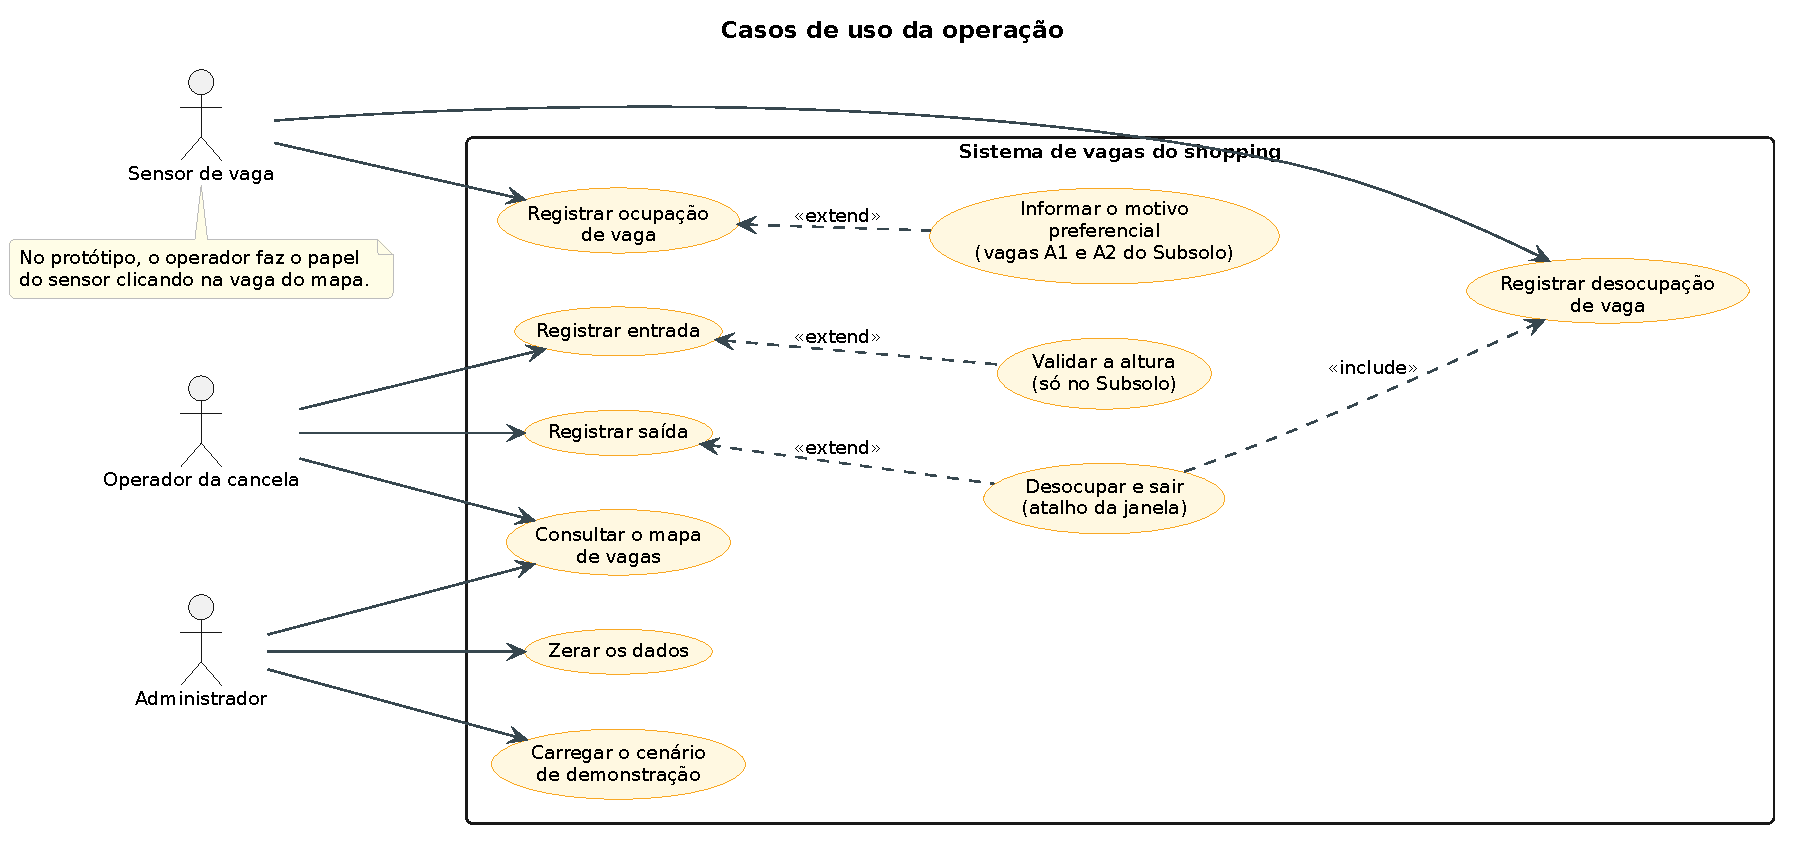
\includegraphics[width=\textwidth]{casos-de-uso-operacao.pdf}
\caption{Casos de uso da operação.}
\label{fig:uc-operacao}
\end{figure}

\begin{figure}[htbp]
\centering
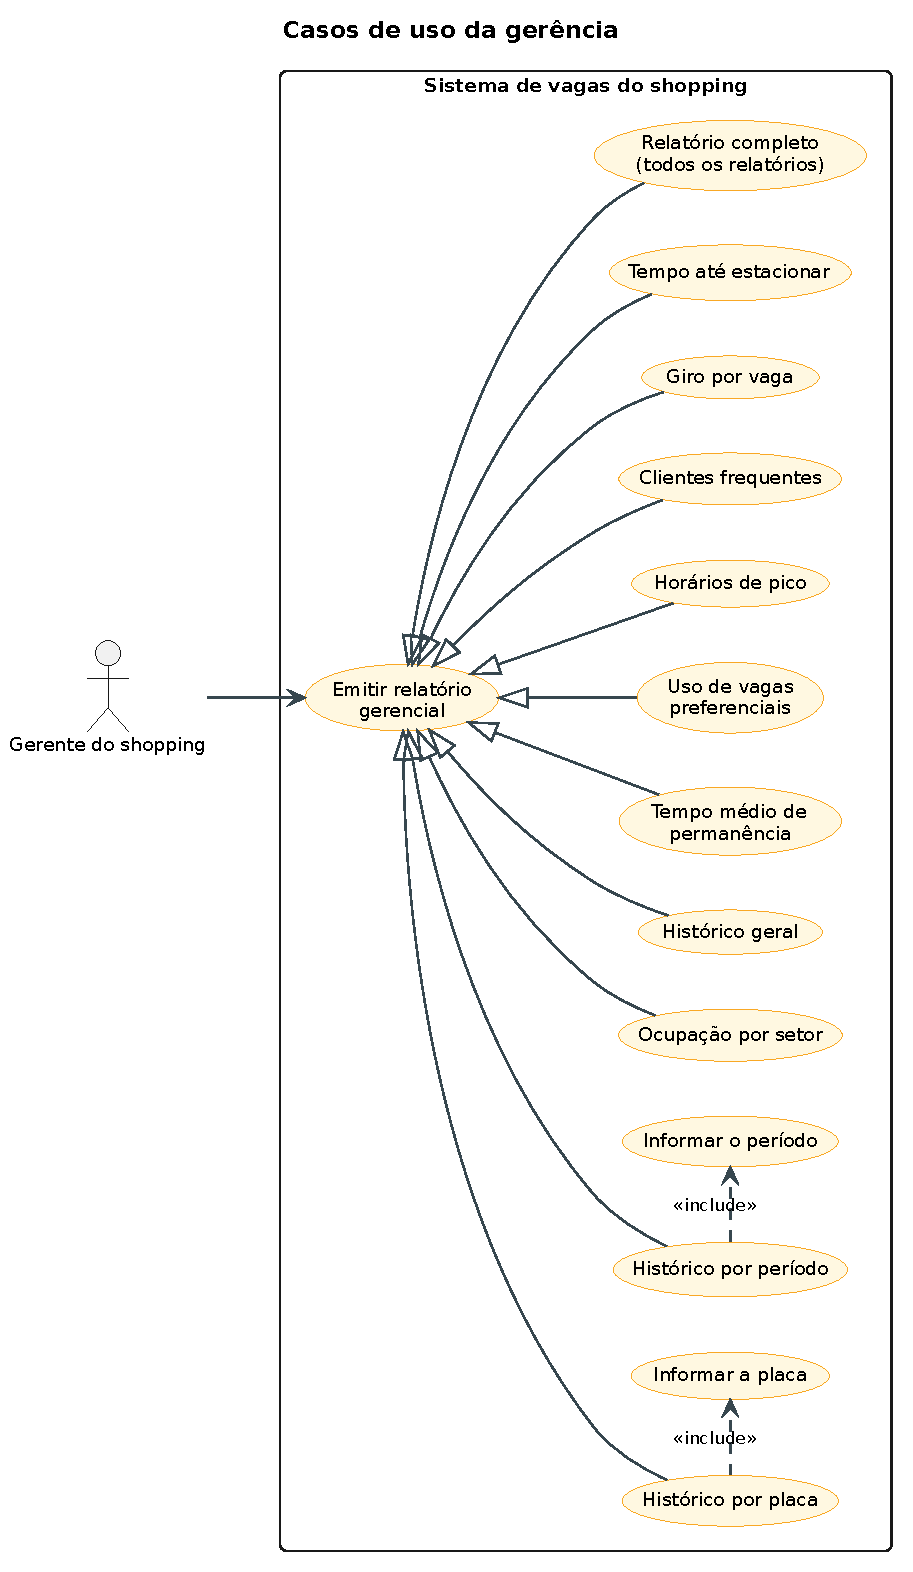
\includegraphics[height=0.6\textheight]{casos-de-uso-gerencia.pdf}
\caption{Casos de uso da gerência.}
\label{fig:uc-gerencia}
\end{figure}

\subsection{Funcional}

O ponto de vista funcional descreve os elementos do sistema em funcionamento, a responsabilidade de cada um e como eles interagem. Os elementos são os três componentes do padrão Blackboard e as peças em volta deles:

\begin{itemize}
  \item o \textbf{quadro} (\texttt{Blackboard}) guarda todo o estado;
  \item o \textbf{controle} (\texttt{BlackboardController}) recebe cada requisição e ativa o primeiro especialista que se declara apto a tratá-la;
  \item os \textbf{especialistas} (\texttt{ExternoKS}, \texttt{SubsoloKS} e \texttt{RelatorioKS}) contêm todas as regras de negócio;
  \item a \textbf{fachada} (\texttt{FachadaEstacionamento}) é o ponto de entrada único das interfaces e da releitura do arquivo;
  \item as \textbf{interfaces} (a janela e a interface de texto) conferem só o formato do que foi digitado (placa de 5 a 8 letras, números ou hífen; altura positiva; data no formato dd/MM/aaaa HH:mm) e mostram o resultado;
  \item o \textbf{registro de eventos} grava no arquivo cada evento aceito.
\end{itemize}

A interação entre eles é sempre a mesma. A interface monta uma requisição e a entrega à fachada; a fachada a publica no quadro e aciona o controle; o especialista escolhido lê o quadro, aplica as regras e escreve o novo estado ou publica a recusa com o motivo; o quadro avisa a janela e o registro de eventos. A Figura~\ref{fig:ciclo} mostra esse ciclo, e os diagramas de atividades detalham cada evento. A Tabela~\ref{tab:regras} reúne as regras que os especialistas de setor aplicam, na ordem em que o código as confere. Uma requisição recusada nunca altera o quadro (P2, P3).

\begin{table}[!htbp]
\centering
\caption{Regras aplicadas pelos especialistas de setor a cada evento.}
\label{tab:regras}
\begin{tabular}{L{2.2cm}L{12.3cm}}
\toprule
\textbf{Evento} & \textbf{Recusado quando\ldots} \\
\midrule
Entrar & a placa está vazia; a placa já está dentro de algum setor; o horário é anterior ao último evento da visita anterior da mesma placa; no Subsolo, a altura não foi informada ou passa de 2,10~m \\
Ocupar & o veículo não entrou neste setor; já ocupa outra vaga; a vaga não existe ou está ocupada; o horário é anterior ao último evento da passagem; numa vaga preferencial, falta o motivo de uso \\
Desocupar & a vaga não existe ou já está livre; o horário é anterior ao último evento da passagem \\
Sair & o veículo não está neste setor; ainda ocupa uma vaga; o horário é anterior ao último evento da passagem \\
\bottomrule
\end{tabular}
\end{table}

A independência dos especialistas (P6) é uma propriedade da estrutura, e não só uma intenção: os especialistas só conhecem o quadro, e o teste automatizado falha se algum deles citar outro. O especialista de relatórios (P5) lê as passagens que os dois setores registraram e calcula os relatórios sem perguntar nada a eles.

\begin{sidewaysfigure}
\centering
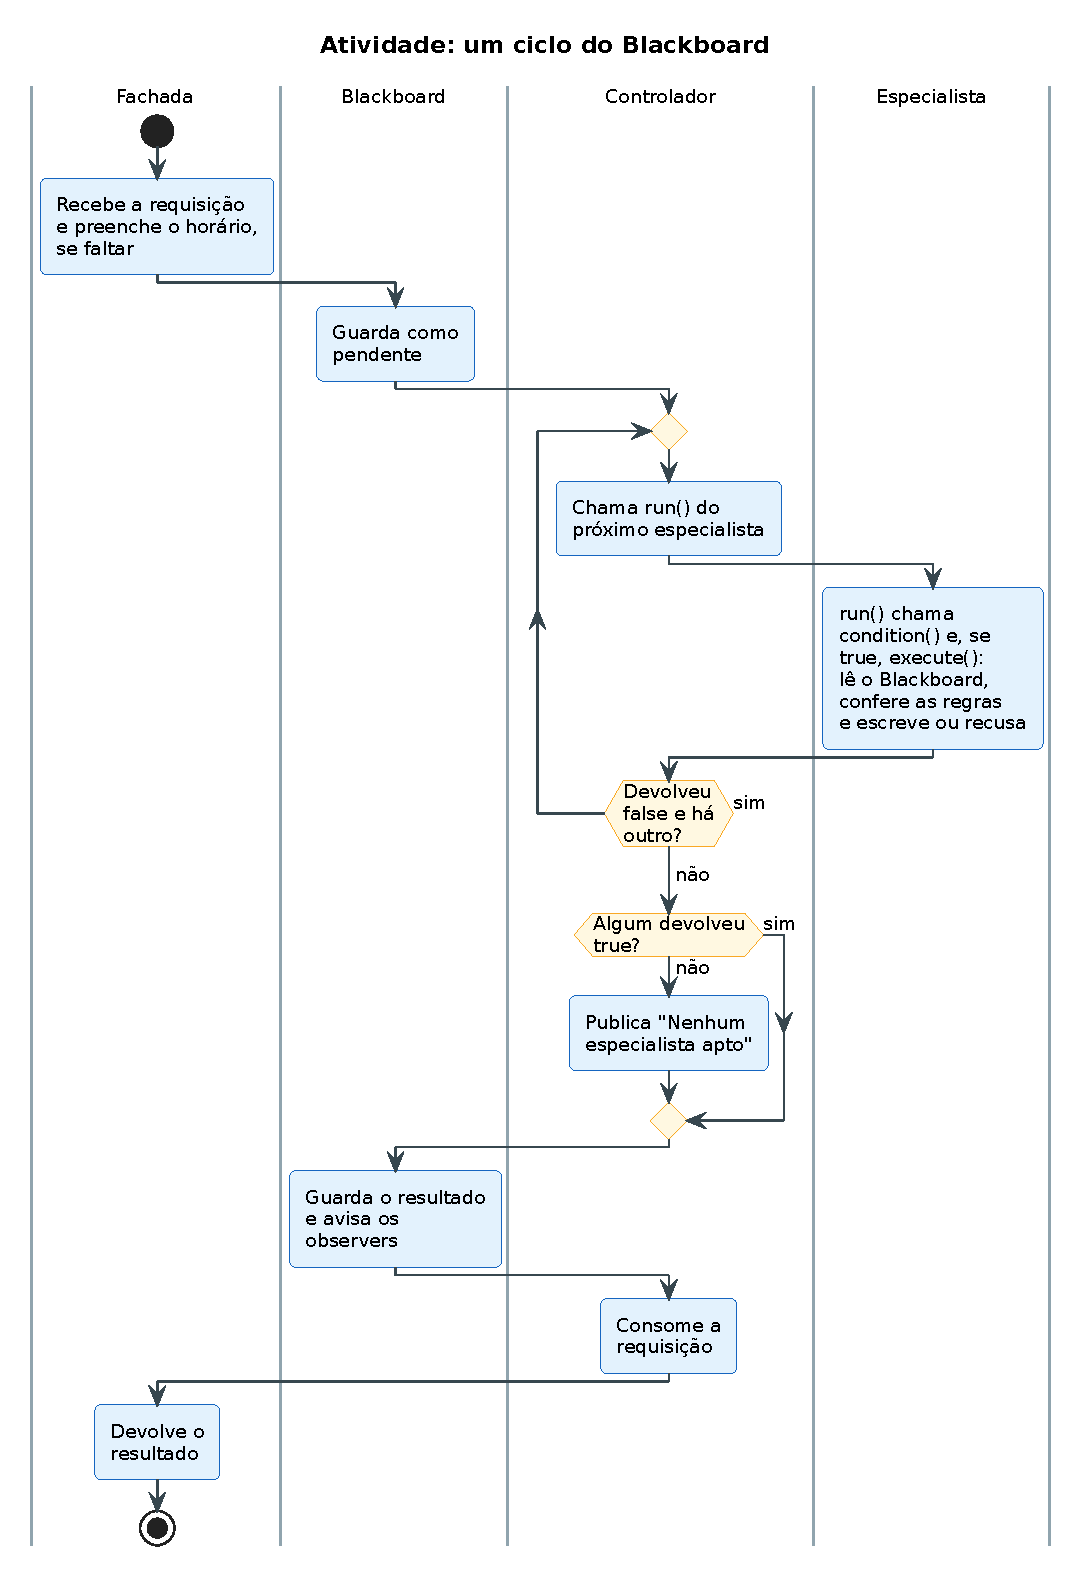
\includegraphics[width=\textheight]{atividade-ciclo-do-blackboard.pdf}
\caption{Atividade: um ciclo do Blackboard, da requisição à resposta.}
\label{fig:ciclo}
\end{sidewaysfigure}

\subsection{Informação}

O ponto de vista de informação descreve como os dados são guardados, transformados e mantidos coerentes. Todo o estado fica no quadro, no modelo da Figura~\ref{fig:modelo}:

\begin{itemize}
  \item cada \textbf{vaga} sabe o setor, a posição, se é preferencial e qual é a ocupação atual, se houver;
  \item cada \textbf{estadia} representa uma passagem de um veículo por um setor: a placa, a altura (no Subsolo), os horários de entrada e saída e a lista de ocupações;
  \item cada \textbf{ocupação} registra a vaga, a placa, o início, o fim e o motivo de uso, quando a vaga é preferencial.
\end{itemize}

\begin{figure}[htbp]
\centering
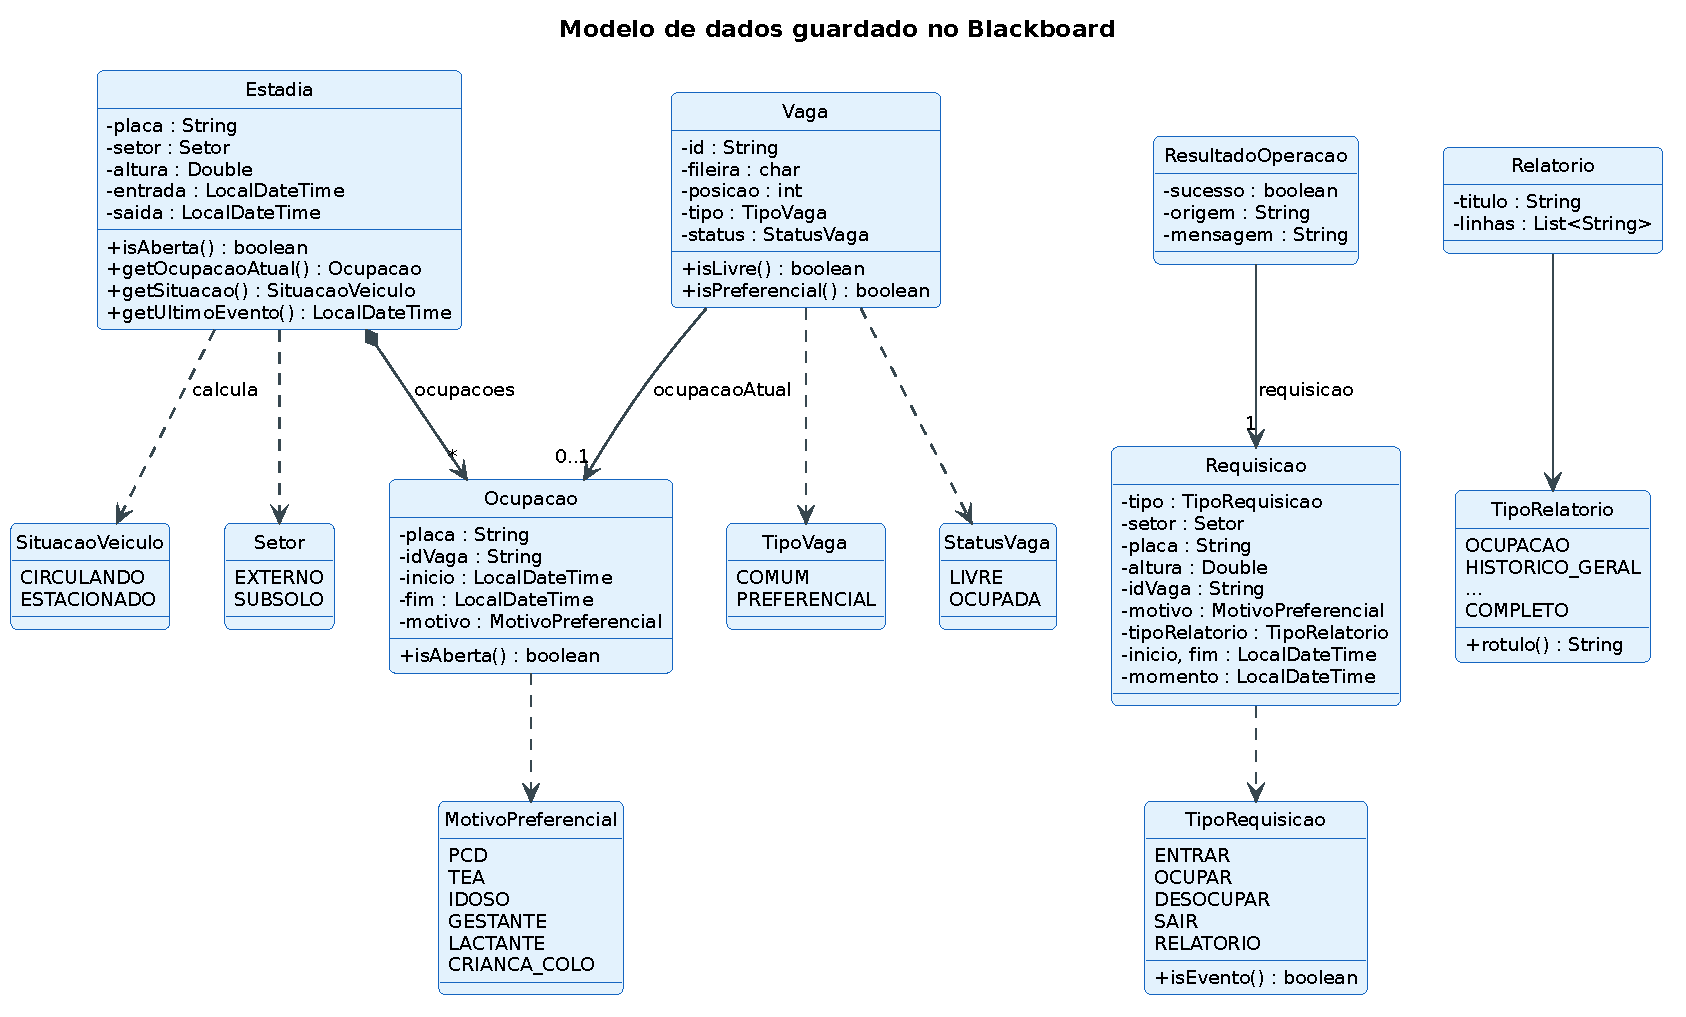
\includegraphics[width=\textwidth]{classes-modelo.pdf}
\caption{Modelo de dados guardado no quadro.}
\label{fig:modelo}
\end{figure}

Três decisões protegem a coerência dos dados (P8):

\begin{itemize}
  \item \textbf{Os estados são calculados, e não guardados em dobro.} A vaga está ocupada quando tem uma ocupação atual; o veículo está estacionado quando a sua estadia tem uma ocupação em aberto (Figura~\ref{fig:estados-veiculo}). Assim, a vaga e o veículo não podem discordar.
  \item \textbf{Cada evento é uma escrita só.} Ocupar uma vaga, por exemplo, liga a vaga à ocupação e acrescenta a ocupação à estadia num único método sincronizado do quadro.
  \item \textbf{Os horários seguem em ordem.} Um evento com horário anterior ao último evento da mesma passagem é recusado, o que protege o histórico (P4).
\end{itemize}

\begin{figure}[htbp]
\centering
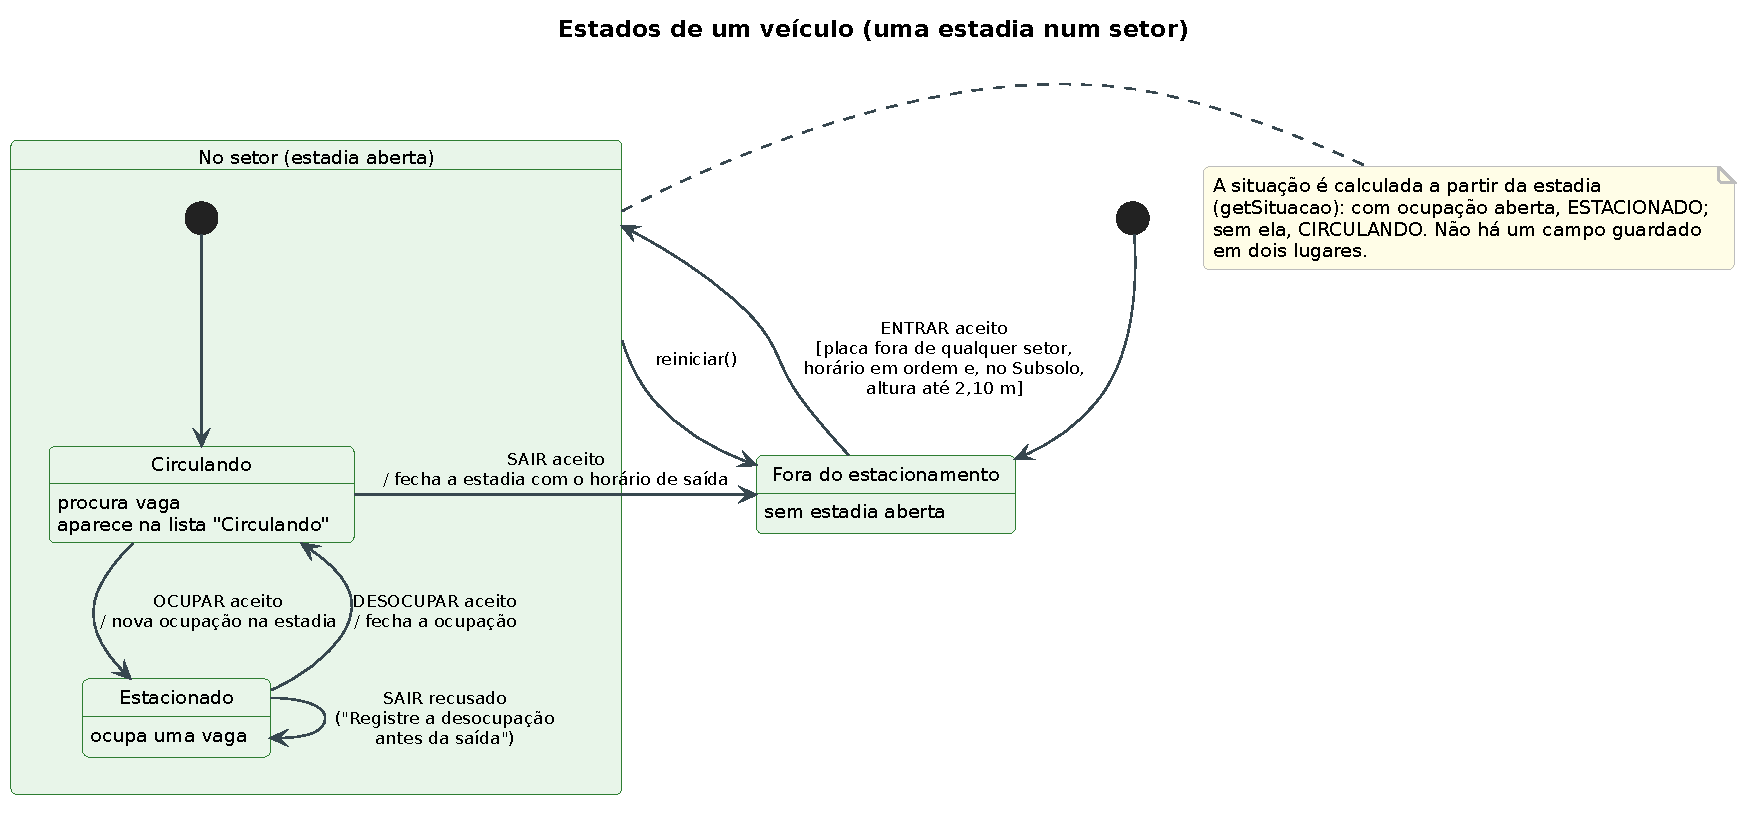
\includegraphics[width=\textwidth]{estados-veiculo.pdf}
\caption{Estados de um veículo durante uma passagem por um setor.}
\label{fig:estados-veiculo}
\end{figure}

Para a durabilidade (P9), o registro de eventos acrescenta uma linha ao arquivo \texttt{dados/eventos.csv} a cada evento aceito, neste formato:
\begin{center}
\texttt{momento;tipo;setor;placa;altura;vaga;motivo}
\end{center}
Ao abrir, o programa relê o arquivo e reenvia cada linha pela fachada, com o horário gravado. Os especialistas reconstroem o quadro aplicando as mesmas regras de uma operação feita na tela, então uma linha adulterada ou fora de ordem é recusada e informada, e não corrompe o estado. O arquivo guarda os \emph{eventos}, e não uma fotografia do estado: o quadro é sempre uma consequência do histórico.

\subsection{Concorrência}

O ponto de vista de concorrência descreve o que acontece ao mesmo tempo e como os conflitos são evitados. O sistema tem três fontes de atividade: a \emph{thread} principal, que relê o arquivo antes de abrir a janela; a \emph{thread} de eventos do Swing, que trata os cliques do operador; e um temporizador do Swing, que redesenha os mapas a cada 30 segundos para atualizar o tempo de espera dos veículos circulando.

Na prática, depois da abertura, quase tudo roda na \emph{thread} do Swing, mas o quadro não depende disso para ficar correto (P8):

\begin{itemize}
  \item todos os métodos do quadro que leem ou escrevem o estado são sincronizados;
  \item o quadro guarda \textbf{uma requisição pendente por vez}, e a fachada só devolve o controle à interface depois que o ciclo termina e a requisição é consumida (Figura~\ref{fig:estados-requisicao});
  \item os avisos aos observadores são feitos fora da trava do quadro, a partir de uma cópia da lista, para que um observador que consulte o quadro durante o aviso não fique bloqueado;
  \item a janela agenda o redesenho na \emph{thread} do Swing, com o método \texttt{invokeLater}, como a biblioteca exige.
\end{itemize}

\begin{figure}[htbp]
\centering
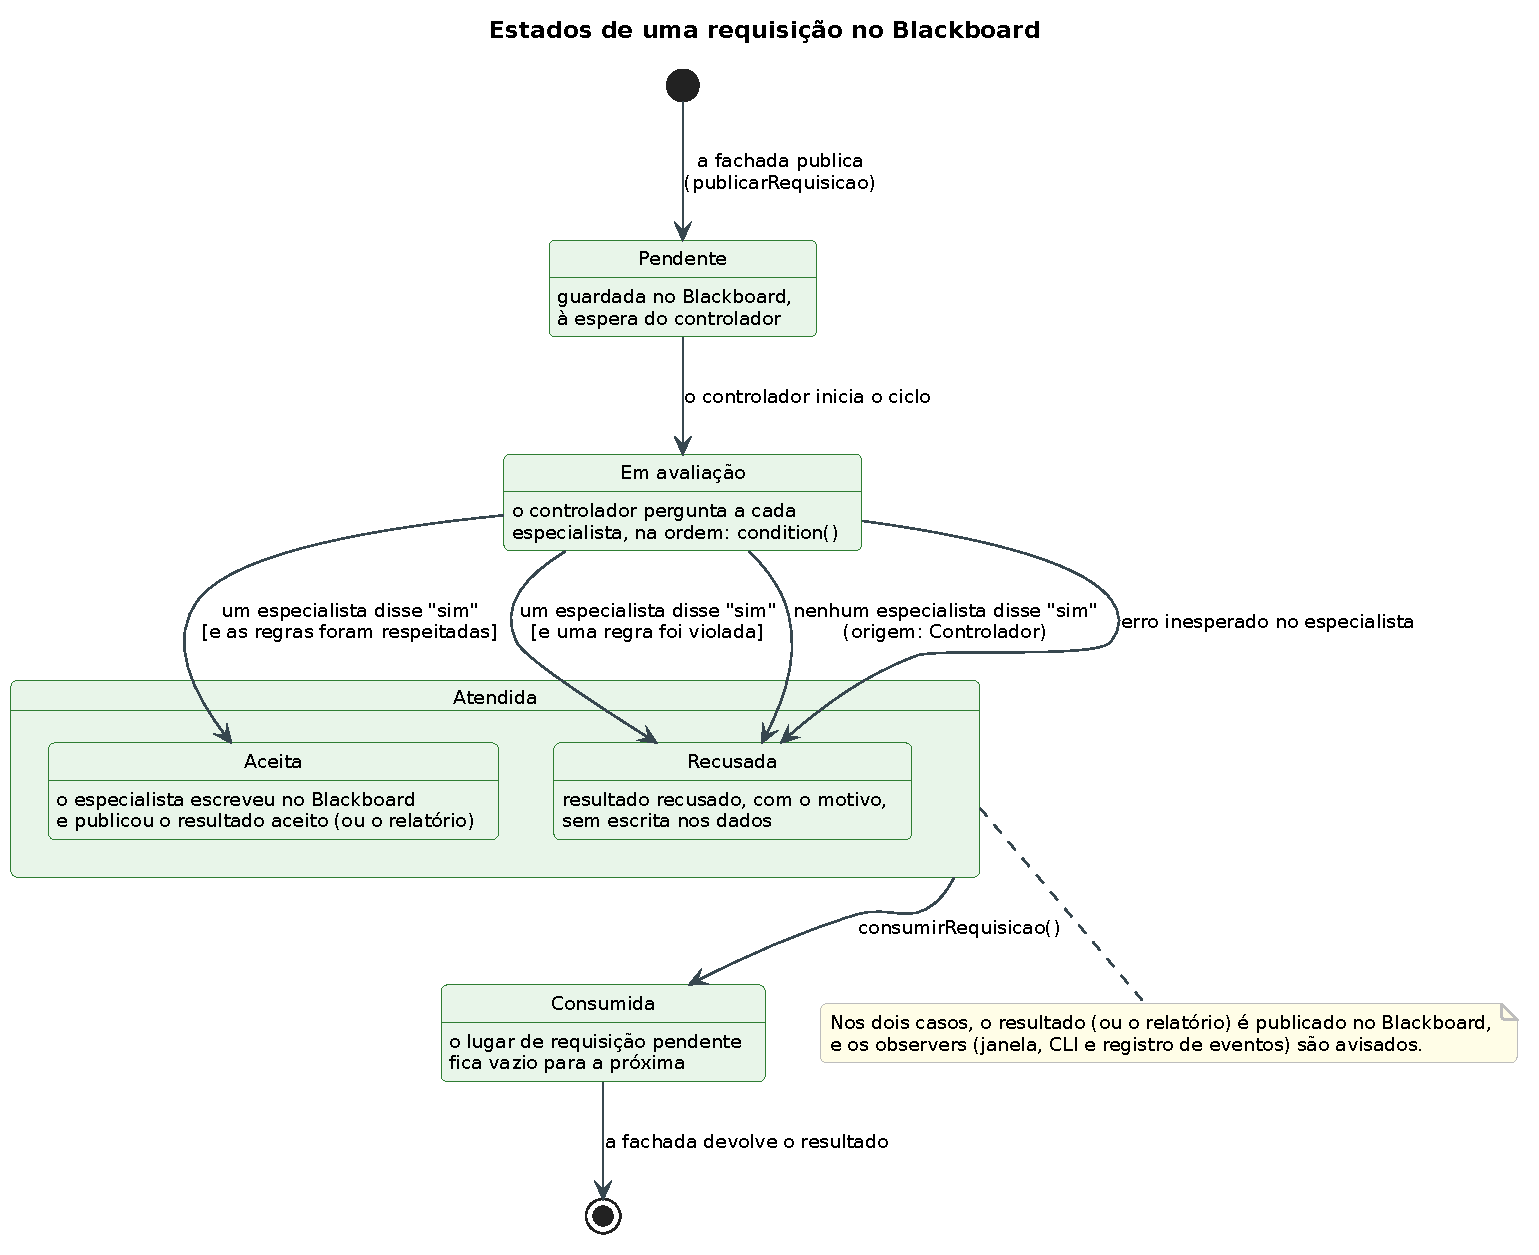
\includegraphics[width=0.8\textwidth]{estados-requisicao.pdf}
\caption{Estados de uma requisição no quadro.}
\label{fig:estados-requisicao}
\end{figure}

\subsection{Desenvolvimento}

O ponto de vista de desenvolvimento descreve como o código é organizado, construído e testado. O código é Java puro, só com a biblioteca padrão do JDK 17 ou mais novo, dividido em pacotes com regras de dependência explícitas (Tabela~\ref{tab:dependencias}). O teste automatizado (\texttt{SmokeTest}) confere essas regras lendo o código-fonte, além dos cenários de cada evento, dos onze relatórios, da gravação e releitura do arquivo e das partes da janela que não dependem da tela (P6, P7).

\begin{table}[!htbp]
\centering
\caption{Pacotes e regras de dependência conferidas pelo teste.}
\label{tab:dependencias}
\begin{tabular}{L{4.0cm}L{4.8cm}L{5.7cm}}
\toprule
\textbf{Pacote} & \textbf{Responsabilidade} & \textbf{Regra} \\
\midrule
\texttt{blackboard} & Quadro e controle & Não importa especialistas, fachada nem persistência \\
\texttt{knowledge\_sources} & Especialistas e cálculos de apoio & Nenhum especialista cita outro, importa a interface ou imprime na tela \\
\texttt{aplicacao} & Fachada & Não importa especialistas \\
\texttt{persistencia} & Registro de eventos e formato CSV & Não importa especialistas \\
\texttt{ui} e \texttt{ui.janela} & Interface de texto e janela & Não importam especialistas nem o controle; únicos a imprimir na tela \\
\texttt{model}, \texttt{util} & Dados e formatação & Sem dependência das camadas acima \\
\bottomrule
\end{tabular}
\end{table}

Para facilitar a demonstração (P11), um único comando (\texttt{./run.sh}) compila e abre o sistema. Duas ferramentas apoiam o desenvolvimento: o gerador do cenário de demonstração, que simula uma semana de uso com semente fixa (o resultado é sempre o mesmo, 2204 eventos de 16 a 22/11/2026, todos com placas fictícias), e uma captura da janela em imagem, usada para conferir o leiaute sem abrir a tela. Os documentos e os diagramas são gerados por um script a partir de textos em LaTeX e PlantUML, guardados no repositório junto com o código.

\subsection{Implantação}

O ponto de vista de implantação descreve onde o sistema roda e do que ele precisa. O protótipo roda num único computador, com Linux, Windows ou macOS, que tenha o JDK 17 ou mais novo (Figura~\ref{fig:implantacao}). Não há servidor, banco de dados nem rede: os módulos rodam na mesma máquina virtual Java, e o estado durável fica em dois arquivos da pasta \texttt{Codigo/dados}, o uso registrado (\texttt{eventos.csv}) e o cenário de demonstração (\texttt{cenario-demonstracao.csv}). As cancelas e os sensores aparecem no diagrama, tracejados, como a integração que um sistema real exigiria.

\begin{figure}[htbp]
\centering
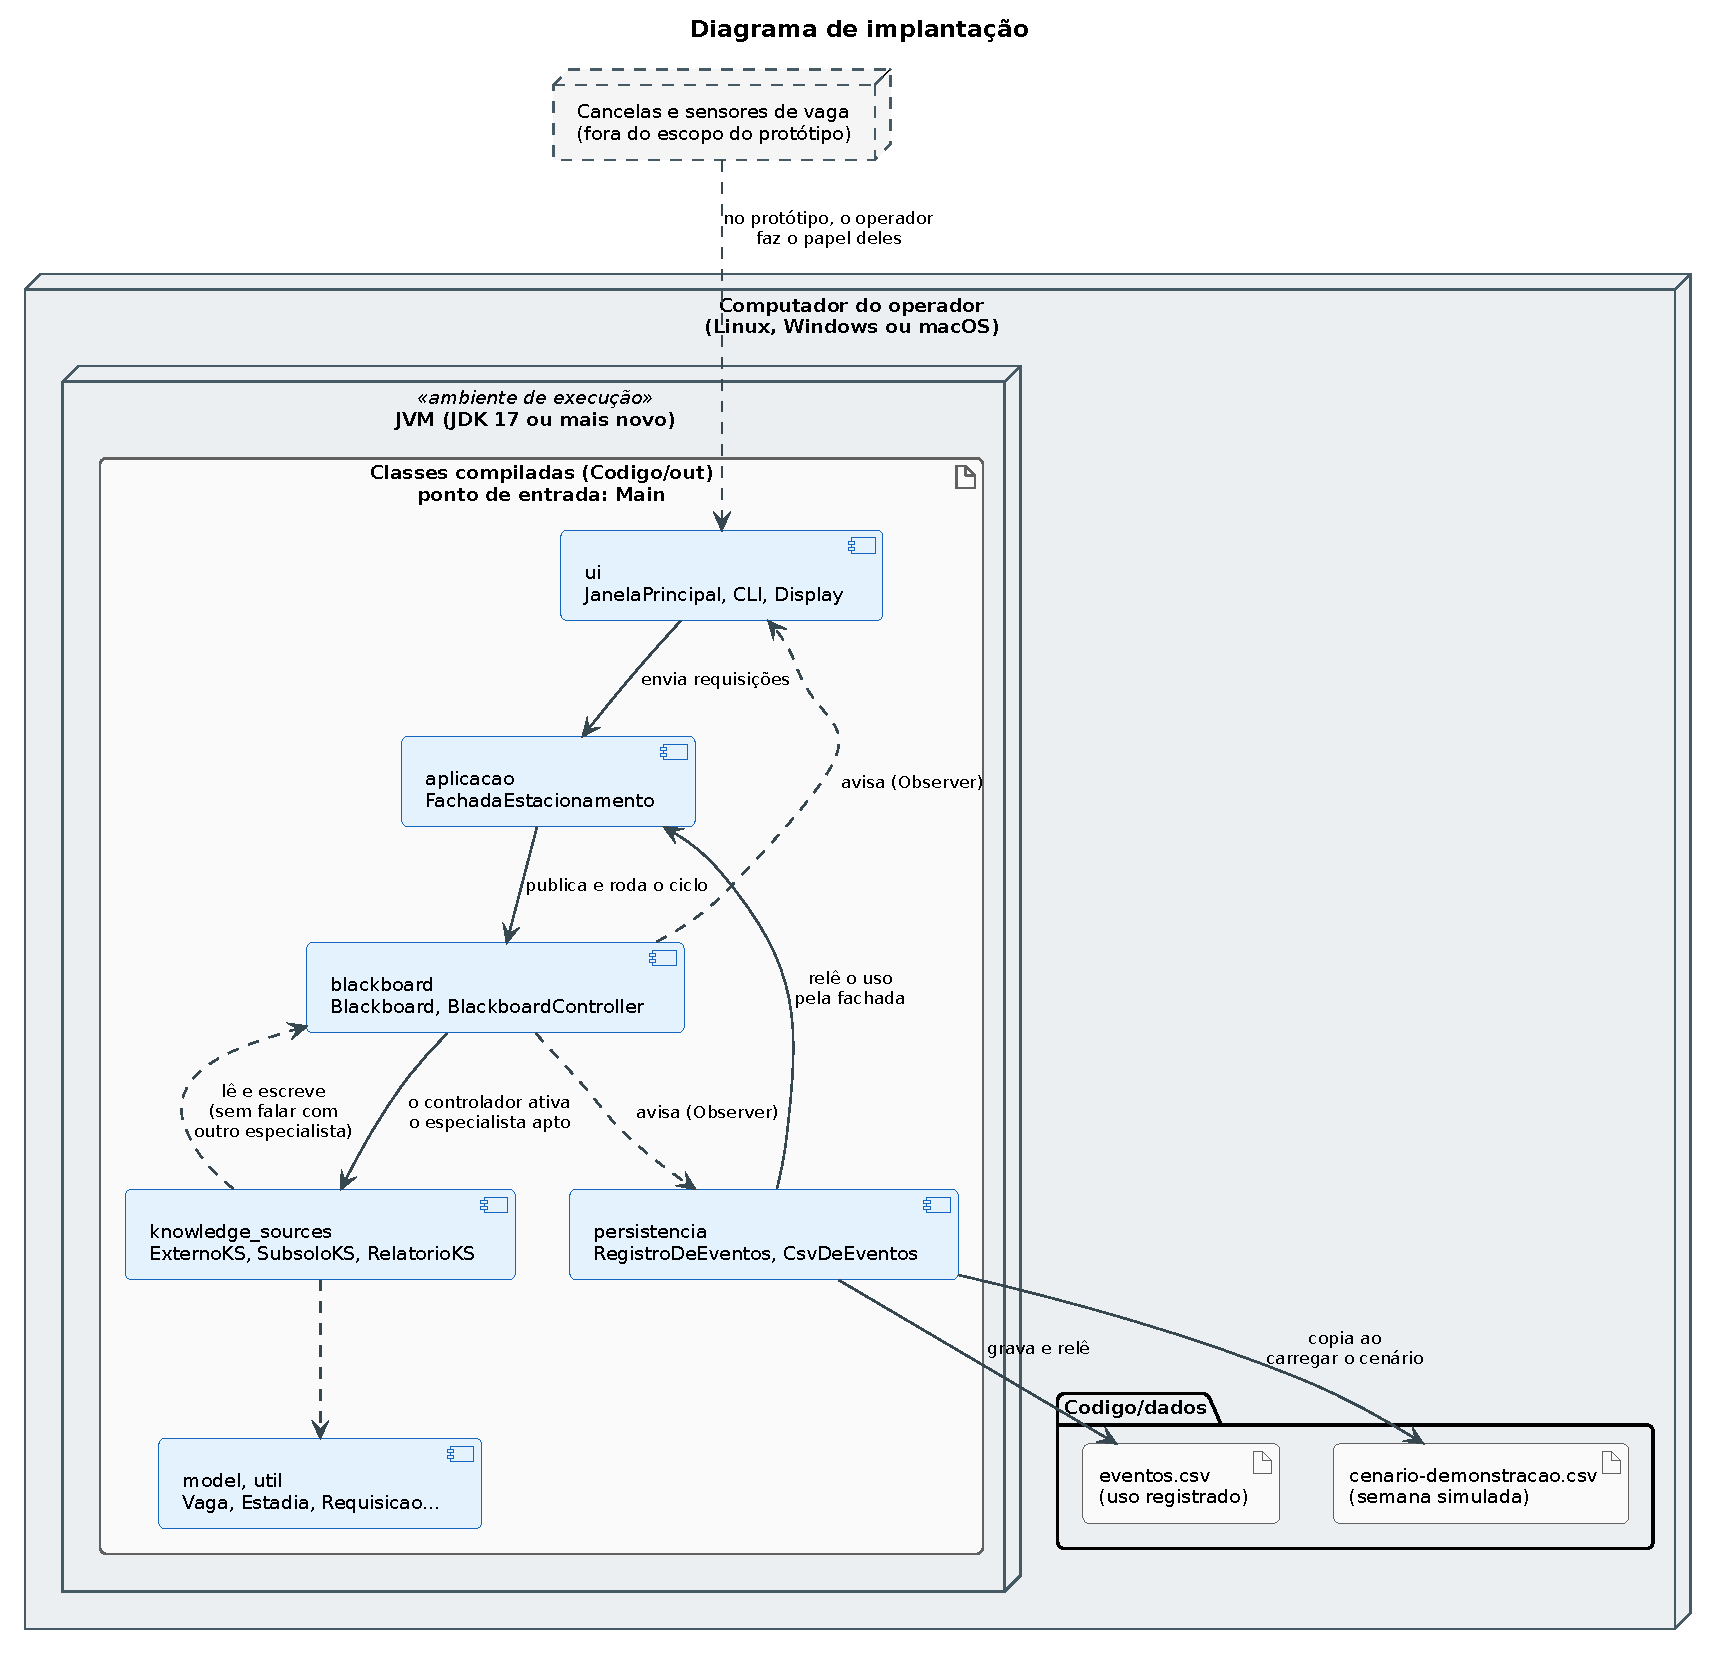
\includegraphics[width=0.9\textwidth]{implantacao.pdf}
\caption{Diagrama de implantação.}
\label{fig:implantacao}
\end{figure}

\subsection{Operacional}

O ponto de vista operacional descreve como o sistema é instalado, posto para funcionar e mantido no dia a dia:

\begin{itemize}
  \item \textbf{Abrir:} \texttt{./run.sh} abre a janela; \texttt{./run.sh --cli} abre a interface de texto. Num computador sem tela gráfica, o sistema abre a interface de texto sozinho e avisa.
  \item \textbf{Carregar o cenário e zerar os dados:} as duas opções ficam no menu ``Dados'' da janela e pedem confirmação, porque substituem o uso registrado. A atividade de carregar o cenário está detalhada no diagrama correspondente.
  \item \textbf{Falhas de gravação:} se o arquivo não puder ser gravado (pasta sem permissão, por exemplo), a operação continua valendo no quadro, e a janela avisa o operador.
  \item \textbf{Linhas inválidas:} ao reler o arquivo, uma linha mal formada ou recusada é pulada, e o resumo da leitura informa o número da linha e o motivo.
  \item \textbf{Cópia de segurança:} basta copiar o arquivo \texttt{eventos.csv}; para restaurar, basta devolvê-lo à pasta e abrir o programa.
\end{itemize}

\section{Perspectivas}
\label{sec:perspectivas}

\subsection{Evolução}

A perspectiva de evolução pergunta o que custa mudar o sistema (P7). Os casos mais prováveis têm caminhos curtos:

\begin{itemize}
  \item \textbf{um terceiro setor} é uma nova subclasse de \texttt{EspecialistaDeSetor}, que só informa o setor e, se precisar, sobrescreve as regras de entrada e de ocupação; ela é acrescentada à lista do controle, e nenhum especialista existente muda;
  \item \textbf{um relatório novo} é um novo tipo na enumeração, um caso no \texttt{switch} do especialista de relatórios e o método que o calcula; se o caso for esquecido, o código não compila;
  \item \textbf{uma interface nova} (uma página web, por exemplo) usa a mesma fachada e se registra como observadora do quadro;
  \item \textbf{um banco de dados no lugar do CSV} troca só o registro de eventos, que já é um observador isolado; os especialistas não sabem onde o histórico é gravado.
\end{itemize}

O que custaria mais é trocar a natureza do controle, por exemplo para vários especialistas candidatos à mesma requisição, com prioridades. A arquitetura comporta essa mudança, mas ela exigiria rever o \texttt{BlackboardController}.

\subsection{Desempenho e escalabilidade}

A perspectiva de desempenho pergunta se o sistema responde a tempo e até onde ele cresce (P12). Com 25 vagas, o estado cabe com folga na memória, e cada operação é uma consulta a poucas listas. A medida mais exigente é a abertura com o histórico: o teste automatizado completo, que relê o cenário de demonstração inteiro (2204 eventos, cada um conferido pelas regras dos especialistas) e roda as demais verificações, termina em menos de um segundo num computador pessoal. A releitura adia os avisos à tela até o fim do lote, para não redesenhar a janela a cada linha.

O limite está no crescimento do histórico. As consultas por placa e por período e os relatórios percorrem a lista de estadias inteira, o que é adequado para semanas ou meses de uso, mas não para anos. Nesse caso, o caminho é o da evolução descrita acima: um banco de dados com índices por placa e por data, atrás do mesmo registro de eventos.

\subsection{Disponibilidade e resiliência}

A perspectiva de disponibilidade pergunta o que acontece quando algo falha (P9). Cada evento aceito é gravado no arquivo no momento em que acontece, então, se o programa for fechado de repente, perde-se no máximo a operação em curso. A releitura é tolerante: uma linha danificada é pulada e informada, e o restante do histórico é recuperado. Se a gravação falhar, o operador é avisado, e a operação continua valendo enquanto o programa estiver aberto. O protótipo não tem redundância: um único computador e um único arquivo. Num sistema real, o arquivo ou o banco ficariam num servidor com cópias de segurança automáticas.

\subsection{Segurança e privacidade}

A perspectiva de segurança pergunta quem pode ver e alterar os dados e como eles são protegidos (P10). Pela Lei Geral de Proteção de Dados (LGPD)~\cite{lei13709}, dado pessoal é a informação relacionada a uma pessoa natural identificada ou identificável. A placa permite identificar o proprietário do veículo por meio de outros cadastros e, por isso, deve ser tratada como dado pessoal. O motivo de uso da vaga preferencial exige ainda mais cuidado: quando ele é ``pessoa com deficiência'' ou ``pessoa com TEA'', a ligação entre a placa e o motivo revela um dado referente à saúde, que a LGPD classifica como \textbf{dado pessoal sensível}.

O protótipo adota três medidas:
\begin{itemize}
  \item \textbf{minimização:} só se guarda o necessário para as regras e os relatórios (placa, altura no Subsolo, horários, vaga e motivo), sem nome, documento ou imagem;
  \item \textbf{dados fictícios no repositório:} o cenário de demonstração usa apenas placas inventadas;
  \item \textbf{uso real fora do repositório:} o arquivo \texttt{eventos.csv}, que guardaria placas reais, é ignorado pelo controle de versões e nunca é publicado.
\end{itemize}

Ficam como limitações, que um sistema real precisaria resolver: não há controle de acesso (quem abre o programa vê e altera tudo), o arquivo não é criptografado, não há prazo de retenção nem eliminação automática dos registros antigos, e o motorista não é informado sobre o tratamento dos seus dados.

\subsection{Usabilidade}

A perspectiva de usabilidade pergunta se as pessoas conseguem usar o sistema sem erro e sem treinamento longo (P1, P11). A janela concentra o essencial numa tela: o mapa de cada setor com uma cor para a vaga livre, outra para a preferencial livre e outra para a ocupada, além da marca ``P'' nas preferenciais, a lista dos veículos circulando com o tempo de espera, os campos da cancela e o painel do ciclo do Blackboard. Quatro escolhas reduzem os erros do operador:

\begin{itemize}
  \item \textbf{as recusas explicam como corrigir} (``registre a entrada antes de ocupar uma vaga''), em vez de só dizer que falhou;
  \item \textbf{o atalho ``desocupar e sair''}: quando a saída é recusada porque o veículo ainda está na vaga, a janela oferece as duas operações de uma vez, e cada uma continua sendo conferida pelo especialista;
  \item \textbf{a ocupação parte do mapa}: ao clicar numa vaga livre, o operador escolhe a placa entre os veículos que estão circulando naquele setor, e não precisa digitá-la de novo;
  \item \textbf{tudo em português}, inclusive os botões das caixas de diálogo, e com o formato de data e de número usado no Brasil.
\end{itemize}

Na interface de texto, quando uma informação é recusada, só ela é pedida de novo, e o restante do que foi digitado é preservado.

\subsection{Regulação}

A perspectiva de regulação pergunta quais leis o sistema precisa respeitar. Além da LGPD, tratada acima, as vagas preferenciais têm base em quatro leis federais:

\begin{itemize}
  \item o \textbf{Estatuto da Pessoa Idosa} (Lei n.º 10.741/2003, art.~41)~\cite{lei10741} assegura às pessoas com 60 anos ou mais a reserva de 5\% das vagas dos estacionamentos públicos e privados, nos termos da lei local, em posição que garanta a melhor comodidade;
  \item o \textbf{Estatuto da Pessoa com Deficiência} (Lei n.º 13.146/2015, art.~47)~\cite{lei13146} exige, nos estacionamentos abertos ao público, vagas próximas aos acessos de pedestres para veículos que transportem pessoa com deficiência com comprometimento de mobilidade: 2\% do total, com no mínimo uma vaga, e o veículo deve exibir a credencial emitida pelo órgão de trânsito;
  \item a \textbf{Lei n.º 12.764/2012}~\cite{lei12764} considera a pessoa com transtorno do espectro autista (TEA) pessoa com deficiência para todos os efeitos legais;
  \item a \textbf{Lei n.º 10.048/2000}~\cite{lei10048} garante atendimento prioritário a pessoas com deficiência, pessoas com TEA, pessoas idosas, gestantes, lactantes, pessoas com criança de colo, entre outras, mas não trata de vagas de estacionamento. A reserva de vagas para gestantes, lactantes e pessoas com criança de colo, quando existe, vem de leis locais ou da política do próprio estabelecimento.
\end{itemize}

O protótipo atende parte dessas exigências e tem limites que precisam ficar claros:

\begin{itemize}
  \item \textbf{Quantidade:} com 25 vagas no total, 5\% equivalem a 1,25 vaga para pessoas idosas, com o arredondamento definido pela lei local, e 2\% equivalem a 0,5 vaga para pessoas com deficiência, o que garante o mínimo de uma. Se a lei local arredondar para baixo, as duas vagas preferenciais do protótipo bastam (uma para cada grupo); se arredondar para cima, seriam necessárias três.
  \item \textbf{Vagas compartilhadas por todos os motivos:} as duas vagas aceitam qualquer um dos seis motivos. Elas não separam as vagas da pessoa idosa das vagas da pessoa com deficiência, como a lei pressupõe, e uma gestante pode ocupar a última vaga livre que uma pessoa com deficiência precisaria.
  \item \textbf{Localização:} as duas vagas preferenciais ficam no Subsolo, que limita a altura a 2,10~m. Um veículo adaptado mais alto, como uma van com elevador para cadeira de rodas, não tem vaga reservada no shopping, porque o Externo não tem vagas preferenciais.
  \item \textbf{Comprovação:} o sistema registra o motivo declarado, mas não confere a credencial exigida pela Lei n.º 13.146/2015; essa conferência continua sendo feita por pessoas.
\end{itemize}

Essa análise foi feita para orientar o protótipo e não substitui uma avaliação jurídica do estacionamento real.

\section{Decisões arquiteturais e alternativas}
\label{sec:decisoes}

A Tabela~\ref{tab:decisoes} registra as decisões que mais influenciaram a arquitetura, com a alternativa considerada e o motivo da escolha.

\begin{table}[!htbp]
\centering
\caption{Decisões arquiteturais.}
\label{tab:decisoes}
\begin{tabular}{L{3.6cm}L{3.8cm}L{7.1cm}}
\toprule
\textbf{Decisão} & \textbf{Alternativa} & \textbf{Motivo} \\
\midrule
Quatro eventos separados (entrar, ocupar, desocupar, sair) & Dois eventos (entrar já ocupando; sair já desocupando) & O enunciado cita os quatro, e a separação permite saber quanto tempo o motorista circula até achar vaga \\
O especialista recusa a saída de um veículo estacionado; a janela oferece o atalho & O especialista desocupar sozinho e registrar a saída & As regras ficam rígidas e explicadas no especialista, e a ajuda fica na tela, que só envia requisições comuns \\
Uma classe-mãe com os fluxos comuns aos setores & Copiar os fluxos em cada setor & As regras comuns ficam num lugar só, sem que um especialista chame o outro \\
Fachada única para as interfaces e a releitura & Cada interface falar com o quadro e o controle & O protocolo do Blackboard não se espalha pelas interfaces \\
Arquivo CSV de eventos, relido pelos especialistas & Banco de dados; ou gravar uma fotografia do estado & Mantém o Java puro, sem biblioteca externa, e cada linha relida passa pelas mesmas regras \\
Estados calculados a partir dos dados & Guardar o estado da vaga e do veículo em campos & O mesmo fato não fica em dois lugares que podem se contradizer \\
Janela em Swing, com a interface de texto mantida & Página web & O Swing já vem no Java; a interface de texto atende terminais sem tela \\
Cenário de demonstração pronto, com semente fixa & Digitar dados durante a apresentação & Relatórios interessantes em segundos, sempre com o mesmo resultado \\
\bottomrule
\end{tabular}
\end{table}

\section{Rastreabilidade até o enunciado}
\label{sec:rastreabilidade}

A Tabela~\ref{tab:rastreabilidade} liga cada exigência do enunciado ao lugar onde ela é atendida.

\begin{table}[!htbp]
\centering
\caption{Rastreabilidade das exigências do enunciado.}
\label{tab:rastreabilidade}
\begin{tabular}{L{6.2cm}L{8.3cm}}
\toprule
\textbf{Exigência} & \textbf{Onde é atendida} \\
\midrule
Arquitetura Blackboard para gerenciar as vagas de um shopping & Pacotes \texttt{blackboard} e \texttt{knowledge\_sources}; Seção~\ref{sec:pontos} e Parte~1 \\
Guardar no quadro a quantidade e a localização das vagas, as ocupadas e as livres, o histórico por placa, os horários e as áreas preferenciais & Classe \texttt{Blackboard} e modelo de dados (Figura~\ref{fig:modelo}) \\
Dois especialistas de setor que atualizam o quadro ao entrar, ocupar, desocupar e sair & \texttt{ExternoKS} e \texttt{SubsoloKS}, com os fluxos em \texttt{EspecialistaDeSetor} (Tabela~\ref{tab:regras}) \\
Um especialista de relatórios com informação útil para a gerência & \texttt{RelatorioKS}, com onze relatórios \\
Especialistas independentes, sem comunicação direta & Regras de dependência conferidas pelo teste (Tabela~\ref{tab:dependencias}) \\
PDF com os padrões de software & Parte~1 (\texttt{padroes-de-software.pdf}) \\
PDF com o problema, o sistema, as preocupações, os pontos de vista e as perspectivas & Este documento \\
Diagrama de implantação & Figura~\ref{fig:implantacao} (\texttt{implantacao.pdf}) \\
Diagramas de casos de uso por tipo de ator & Figuras~\ref{fig:uc-operacao} e~\ref{fig:uc-gerencia} \\
Diagramas de atividades & Figura~\ref{fig:ciclo} e os cinco diagramas \texttt{atividade-*.pdf} \\
Diagramas de estados, se houver máquina de estados & Vaga, veículo e requisição (\texttt{estados-*.pdf}) \\
Front-end simples para demonstrar a arquitetura & Janela Swing e interface de texto, abertas com \texttt{./run.sh} \\
\bottomrule
\end{tabular}
\end{table}

\section{Limitações}
\label{sec:limitacoes}

Além dos limites apontados nas perspectivas, o protótipo tem estas limitações conhecidas:

\begin{itemize}
  \item as cancelas, os sensores e a leitura de placas são simulados pelo operador;
  \item roda num único computador, sem uso simultâneo em rede;
  \item não há controle de acesso, criptografia do arquivo nem política de retenção dos dados;
  \item as duas vagas preferenciais atendem a todos os motivos, ficam só no Subsolo e não conferem a credencial;
  \item a configuração das vagas (quantidade, posição e preferenciais) está fixa no código;
  \item as consultas percorrem todo o histórico, o que limita o volume de dados a semanas ou meses de uso.
\end{itemize}

\section{Conclusão}

O sistema resolve os cinco problemas do estacionamento com um quadro central e três especialistas independentes: o mapa mostra as vagas livres em tempo real, a altura e o motivo de uso das preferenciais são conferidos pelos especialistas, a gerência tem onze relatórios e o histórico sobrevive em arquivo. Os sete pontos de vista mostram como cada preocupação das partes interessadas é tratada na estrutura, e as perspectivas deixam claros os limites do protótipo, sobretudo na privacidade dos dados e na regulação das vagas preferenciais, que um sistema real precisaria tratar antes de entrar em uso.

\bibliographystyle{plain}
\bibliography{referencias}

\end{document}
